%%%%%%%%%%%%%%%%%%%%%%%%%%%%%%%%%%%%%%%%%%%%%%%%%%%%%%%%%%%%%%%%%%%%%%%%%%%%%%%%
%2345678901234567890123456789012345678901234567890123456789012345678901234567890
%        1         2         3         4         5         6         7         8

\documentclass[letterpaper, 10 pt, conference]{ieeeconf}  % Comment this line out if you need a4paper

% \documentclass[a4paper, 10pt, conference]{ieeeconf}      % Use this line for a4 paper

% \IEEEoverridecommandlockouts                              % This command is only needed if 
                                                          % you want to use the \thanks command

\overrideIEEEmargins                                      % Needed to meet printer requirements.

% See the \addtolength command later in the file to balance the column lengths
% on the last page of the document

% The following packages can be found on http:\\www.ctan.org
\usepackage{graphics} % for pdf, bitmapped graphics files
\usepackage{epsfig} % for postscript graphics files
%\usepackage{mathptmx} % assumes new font selection scheme installed
%\usepackage{times} % assumes new font selection scheme installed
%\usepackage{amsmath} % assumes amsmath package installed
%\usepackage{amssymb}  % assumes amsmath package installed

\title{\LARGE \bf
A Novel Control Architecture for Complex Robot Tasks
}


\author{Luke Fraser$^{1}$ and Monica Nicolescu$^{2}$% <-this % stops a space
%\thanks{*This work was not supported by any organization}% <-this % stops a space
\thanks{$^{1}$Luke Fraser is a graduate student in the Department of Computer Science and Engineering,
        University of Nevada, Reno
        {\tt\small Fraser@Nevada.unr.edu}}%
\thanks{$^{2}$Monica Nicolescu is a Professor with the Department of Computer Science and Engineering, University of Nevada, Reno
        {\tt\small monica@unr.edu}}%
}


\begin{document}



\maketitle
\thispagestyle{empty}
\pagestyle{empty}

%%%%%%%%%%%%%%%%%%%%%%%%%%%%%%%%%%%%%%%%%%%%%%%%%%%%%%%%%%%%%%%%%%%%%%%%%%%%%%%%
\begin{abstract}
Robot tasks for real-world applications typically involve multiple paths of execution, when the same task could be achieved in multiple different ways. This poses challenges with respect to the representation and execution of such tasks, as enumerating all possible execution paths leads to combinatorial increases in the represntation. In this paper we present a novel robot control architecture that addresses these challenges. The architecture 1) provides an efficient, compact encoding of tasks with multiple paths of execution, 2) it uses the same compact representation as the controller that the robot will use to achieve its goals and 3) it allows the robot to dynamically decide which execution path to follow using an activation spreading mechanism that relies on environmental conditions. We validate our architecture using a humanoid Baxter robot, showing that the robot dynamically selects a path of execution, based on the current state of the environment.

\end{abstract}


%%%%%%%%%%%%%%%%%%%%%%%%%%%%%%%%%%%%%%%%%%%%%%%%%%%%%%%%%%%%%%%%%%%%%%%%%%%%%%%%
\section{INTRODUCTION}


%%%%%%%%%%%%%%%%%%%%%%%%%%%%%%%%%%%%%%%%%%%%%%%%%%%%%%%%%%%%%%%%%%%%%%%%%%%%%%%%
In real-world applications, the tasks that a robot would have to complete are typically more complex than a sequence of steps that must be performed in order. Furthermore, the same task could be performed in a wide variety of ways, due in large part to the affordances present in the environment. As an example, an assembly task may have parts during which some steps must be executed sequentially (i.e, an axle must be mounted before the wheel), other parts in which the steps could be executed in any order (i.e., mounting four wheels could happen in any order), and also parts that could be achieved through multiple paths of execution (i.e, could use either wrench1 or wrench2 to tighten the bolts). The tasks could further be structured using a hierarchical representation. The robot's task representation and the underlying control architecture should enable the representation of all these constraints and alternate options, in order to allow the robot flexibility in performing the task. 

To date, the general approach for encoding robot controllers relies on a relatively fixed representation, which restricts the robot to always performing a task using a pre-defined, fixed sequence of steps. Several recent approaches for encoding such complex activities have been developed \cite{koppula2013anticipating}\cite{hawkins2014anticipating}, which have been successfully demonstrated on typically small-scale tasks. The major challenge for encoding tasks with {\it no ordering constraints} on their steps and with {\it multiple paths of execution} leads to a combinatorial increase in the representation, due to the fact that all possible execution paths need to be explicitly encoded in the architecture. While the tasks can in principle be encoded using a compact representation, the robot controller needs to expand that to its for actual robot execution. In this paper we propose a robot control architecture that enables both a {\it compact encoding} and {\it execution} of the above tasks. Furthermore, through the use of an activation spreading mechanism, the representation allows the robot to dynamically decide which path of execution to follow. The architecture follows a behavior-based paradigm, in which basic robot capabilities are represented as nodes in an interconnected network. 

The remainder of this paper is structured as follows: Section~\ref{relatedWork} describes previous related research, Section~\ref{architecture} presents our approach for encoding and executing complex tasks, Section~\ref{evaluation} shows our experimental evaluation and Section~\ref{conclusion} gives a summary of the presented work.
%[32]	Koppula, H. S., and A. Saxena, 2013, Anticipating Human Activities using Object Affordances for Reactive Robotic Response: Robotics Science and Systems.

%[36]	Hawkins, K.P.; Bansal, S.; Vo, N.N.; Bobick, A.F., "Anticipating human actions for collaboration in the presence of task and sensor uncertainty," Robotics and Automation (ICRA), 2014 IEEE International Conference on , vol., no., pp.2215,2222, May 31 2014-June 7 2014
%%%%%%%%%%%%%%%%%%%%%%%%%%%%%%%%%%%%%%%%%%%%%%%%%%%%%%%%%%%%%%%%%%%%%%%%%%%%%%%%
\section{Related Work}
\label{relatedWork}

% Add intro sentence.
Recent work  addresses these challenges using a probabilistic approach for predicting human actions and a cost based planner for the robot’s response [38]. Tasks are represented as Bayes networks and prediction of human actions is performed using a forward-backward message passing algorithm in the network. This inference process is however dependent on knowledge of the full conditional probability table for the task, which increases computational complexity for large tasks and limits adaptability to changes in the task at run-time. This work has been expanded in [39], with a new task representation that can encode tasks with multiple paths of execution. The initial representation for the task is a compact AND-OR tree structure, but for action prediction and planning, it has to be converted into an equivalent Bayes network, which has to explicitly enumerate all possible alternative paths. 
%[38]	K. Hawkins, N. Vo, S. Bansal, A. Bobick, “Probabilistic human action prediction and wait-sensitive planning for responsive humanrobot collaboration”, Proceedings of the IEEE-RAS International Conference on Humanoid Robots, 2013.
%[39]	Hawkins, K.P., Bansal, S., Vo, N.N., Bobick, A.F., “Anticipating human actions for collaboration in the presence of task and sensor uncertainty,” IEEE International Conference on Robotics and Automation (ICRA), pp.2215-2222, 2014.
%Scaz paper
% Hierarchical approaches
\section{Proposed Archictecture}
\label{architecture}
\subsection{Task Representation}
\label{representation}
The control architecture we present below serves three main roles: 1) it provides an efficient, compact encoding of tasks that have sequential, non-ordering and alternative paths of execution, 2) it allows the use of this compact representation to execute the robot's goals and 3) it allows the robot to dynamically decide which execution path to follow using an activation spreading mechanism that relies on environmental conditions.

We developed our representation using a behavior-based paradigm \cite{arkin1998behavior}, which provides modularity and ease in communication and connectivity between behavioral modules.  As previously mentioned, our aim is to enable the system to encode tasks that involve temporal sequencing constraints (some steps need to happen before others), alternative ways of execution (any one of multiple options is acceptable), and no temporal constraints (some steps can be executed in any order). All these options could be a part of a single task representation, which could be seen from a task such as "a {\bf THEN} ((b {\bf THEN} c) {\bf AND} (d {\bf OR} e {\bf OR} (f {\bf THEN} g)))". To encode such a task we will define two types of nodes in our behavior network. Behavior nodes encode a basic behavior that achieves a well-defined goal (such as a, b, c, d, e, f, g above). Goal nodes are N-ary trees (i.e., can have from 0 to N children) and encode the three different types of execution constraints mentioned above, as follows:
\begin{itemize}

\item {\bf THEN} goal nodes encode sequencing constraints. For example, GoalSeq = a {\bf THEN} b, implies that in order to achieve GoalSeq, the system should execute basic behavior a, followed by behavior b.

\item {\bf OR} goal nodes encode alternate paths of execution. For example GoalAlt = a {\bf OR} b, implies that in order to achieve GoalAlt, the system can execute either behavior a or behavior b.

\item {\bf AND} goal nodes encode the option of having no ordering constraints. For example GoalNoOrd = a {\bf AND} b, implies that in order to achieve GoalNoOrd, the system should execute both behaviors a and behavior b, but in any order. This also leads to alternative paths of task execution, but in which all the individual components must be performed at some point.

\end{itemize}
%[12]	R. C. Arkin, Behavior-Based Robotics, MIT Press, CA, 1998.

% For one-column wide figures use
\begin{figure}
\centering
  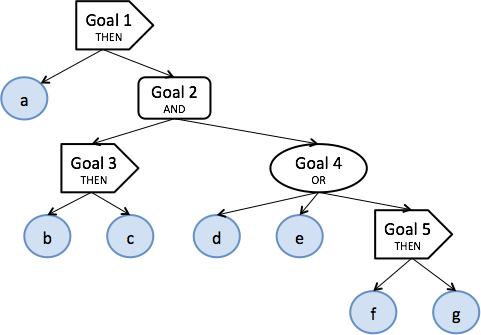
\includegraphics[width=6cm]{task_img.png}
\caption{Representation of task "a {\bf THEN} ((b {\bf THEN} c) {\bf AND} (d {\bf OR} e {\bf OR} (f {\bf THEN} g)))"}
\label{fig:task_representation}       % Give a unique label
\end{figure}
%This needs updating
With these types of components, the above task will be represented as shown in Figure~\ref{fig:task_representation}. A task could have any type of goal node as a root and there is no restriction on which nodes could be parents of others in the hierarchy. It can be seen that this representation compactly encodes all the task constraints, including all possible paths of execution. This is especially important when there are multiple alternative paths, such as for Goal2: either Goal3 or Goal4 could be performed first; to achieve Goal4, either one of d, e or Goal5 could be executed. Instead of explicitly enumerating all possibilities [36], we use the most compact form of the task representation. This representation would be more accurately represented by the following prefix encoding: (THEN a, (AND (THEN b c) (OR d e (THEN f g)))).

\subsection{Controller Implementation}
\label{implementation}
%Luke: this may actually fit under the next subsection

\subsection{Task Execution}
\label{execution}

Each goal node stores the following information: status (indicates whether the goal has been achieved, not achieved but currently being worked on, or not achieved and not actively being pursued), type (THEN, OR, AND) and activation level. During task execution, each goal node continuously evaluates its status (computed from the status of its children) and this information is available for the higher-level parent nodes. To perform a task, a robot would use the above task representation as follows: the root node of the task (typically a goal node) evaluates if all its children goal/behavior nodes are met. If they are, nothing needs to be done. Otherwise, the node will send activation messages to its children nodes in order to signal that they should be met. These goal nodes, in turn, send activation messages as needed to their children. Messages are also passed from children nodes that are currently active (basic behaviors that are running, or goal nodes that are actively being pursued) upwards to the parents to indicate that the current goal is under execution. This is important for keeping track of which pathways of execution and goals are currently under execution and is a key feature that enables seamless self-organization within the robot team (Section 3.2). The different types of goal nodes send activation messages to their children as follows:

\begin{itemize}

\item {\bf THEN} goal nodes evaluate the status of their children in the order given by the sequence and send activation messages with decreasing magnitudes, from the first goal in the list whose status is not met to the last. This ensures that the subsequent steps of the task are already primed for execution as soon as the current step is done, as well as permitting other robots to prepare for and be ready to help or take over the next step, as explained in Section 3.2.  

\item {\bf OR} goal nodes initially send activation messages to all their children. Once the activation messages reach a leaf node (basic behavior), the behavior with the highest activation level and whose own preconditions are met will start running. This allows for opportunistic task execution, in situations in which environmental conditions are met for just one (or some) of the alternative pathways. In case of equal activation levels and applicability conditions, the robot will choose one of the options at random. Once a pathway becomes active (detected through messages from the children), the goal node will stop sending activation messages to all the other children.

\item {\bf AND} goal nodes send activation messages to all their children. When a particular child node becomes active, the node will increase the activation it is sending to the active child, but continue sending activation to the other children nodes. This would ensure that the system would not oscillate between a child goal node to another.
\end{itemize}

% \addtolength{\textheight}{-15cm}   % This command serves to balance the column lengths
                                  % on the last page of the document manually. It shortens
                                  % the textheight of the last page by a suitable amount.
                                  % This command does not take effect until the next page
                                  % so it should come on the page before the last. Make
                                  % sure that you do not shorten the textheight too much.
\section{Experimental Evaluation}
\label{evaluation}

We evaluated our work using a Baxter humanoid robot working on the task of setting up a dinner table. The objects that the robot can use for this task include: fork, spoon, knife, wine glass, cup, soda can, place mat, plate, and salad plate. We created a task representation that encapsulates all the constraints that occur in such a scenario, as shown in Figure~\ref{fig:set_table}. 

\begin{figure}
\centering
  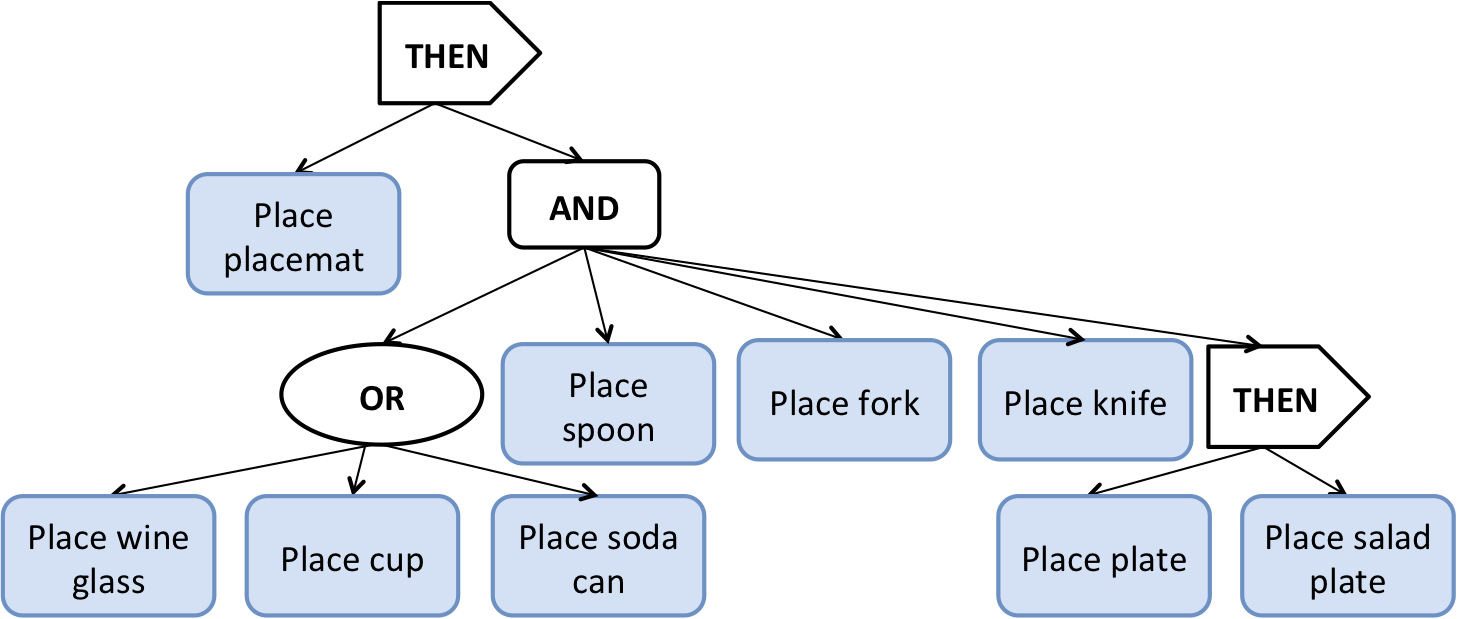
\includegraphics[width=6cm]{set_table_task.png}
\caption{Task representation for setting up the table}
\label{fig:set_table}       % Give a unique label
\end{figure}

As shown, the task structure encodes sequential constraints (e.g., setting up the place mat before the plate), alternative paths of execution (e.g., choose either the wine glass, the cup or the soda can) and steps whose ordering is not important (e.g., placing the spoon, the fork and one of the drinking objects). For evaluation, we created three different setups, in which the objects are placed at different locations on the table. At execution time, the robot uses the locations of the objects and its activation spreading mechanism to dynamically decide which parts of the task to perform. As currently implemented, the objects that are closer will have a higher activation level than objects farther away, so the robot will choose to first handle the objects that are at a smaller distance, while still maintaining the ordering constraints represented in the task structure. Figure~\ref{fig:setup} shows our experimental environment.

%Luke: take a picture of the environment and include it here
% \begin{figure}
% \centering
%   \includegraphics[width=6cm]{setup.png}
% \caption{Experimental setup}
% \label{fig:setup}       % Give a unique label
% \end{figure}

For each experiment we recorded the following information: 1) the activation level for each low-level behavior throughout the duration of the experiment and 2) the times during which the behaviors were active. Figure~\ref{fig:results} show the results for each of the three scenarios. As seen from the plots with the activity of behavior, the robot chose different ways of achieving the same task, while obeying the constraints set in the task representation. The results show that with the same compact network structure, solely through the activation spreading mechanism, the robot can select on its own way of accomplishing the task.

%Luke: I thought we can structure this as a 2 row by 3 column matrix: top row shows the activation levels, bottom row shows the behaviors running
% \begin{figure}
% \centering
%   \includegraphics[width=6cm]{results.png}
% \caption{Results of the three experimental setups: a) Setup 1, b) Setup 2, c) Setup 3}
% \label{fig:results}       % Give a unique label
% \end{figure}

\section{Conclusion}
\label{conclusion}
In this paper we presented a new control architecture that allows for efficient encoding of tasks with multiple way of execution. The representation used for encoding the task structure serves at the same time as a controller that the robot can use for executing the task. Based on this task representation and an activation spreading mechanism within the nodes of the task, the robot can dynamically select which path of execution to perform, based on the current environmental conditions. We validated our approach on a physical humanoid Baxter robot, working on the task of setting the table, in different scenarios that resulted in different ways of execution for the task.

\bibliographystyle{IEEEtran}
\bibliography{refs/master.bib}
%%%%%%%%%%%%%%%%%%%%%%%%%%%%%%%%%%%%%%%%%%%%%%%%%%%%%%%%%%%%%%%%%%%%%%%%%%%%%%%%
%\section*{APPENDIX}

%\section*{ACKNOWLEDGMENT}

%%%%%%%%%%%%%%%%%%%%%%%%%%%%%%%%%%%%%%%%%%%%%%%%%%%%%%%%%%%%%%%%%%%%%%%%%%%%%%%%
\end{document}
